\section{Tiered Compilation in Hotspot}
As mentioned in the introduction, Programming Language Virtual Machines like Java Hotspot feature a multi-tier system when compiling methods during execution. 
Java VM's typically use Java Bytecode as input, a platform independent intermediate code generated by a Java Compiler like \texttt{javac}.
The Bytecode is meant to be interpreted by the virtual machine or further compiled into platform dependend machine code.
Hotspot includes one interpreter and two different compilers with different profiling levels resulting in a total of 5 different levels. The following Figure \ref{fig:hs_tiers} gives a short overview as well as showing the standard transitions.
\begin{figure}[h]
  \begin{center}
    \centering
    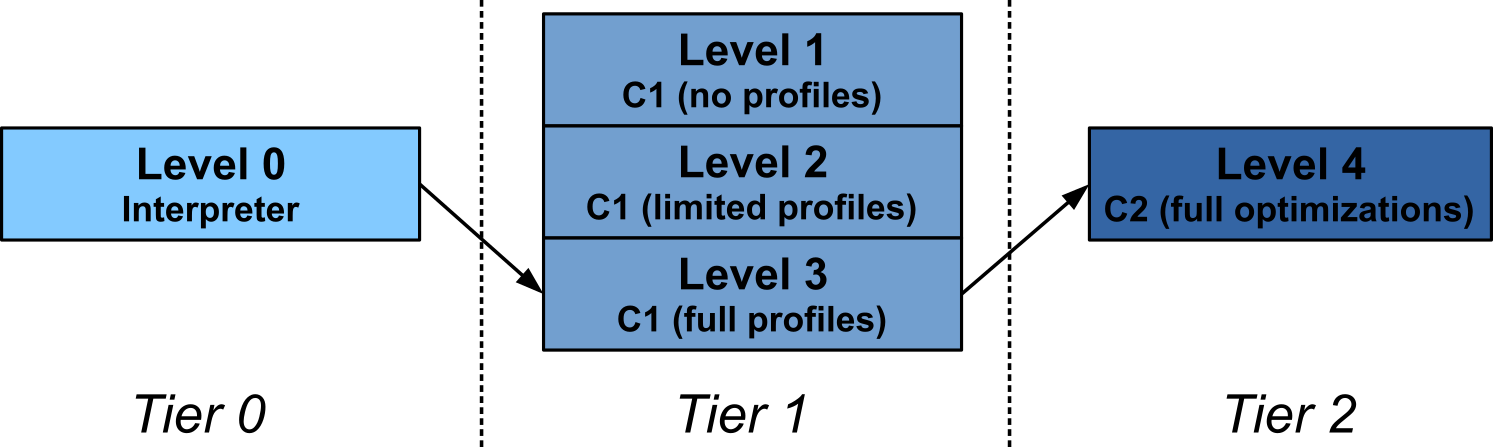
\includegraphics{figures/hs_tiers.png}
    \caption{Overview over compilation tiers}
    \label{fig:hs_tiers}
  \end{center}
\end{figure}

All methods start being executed by Tier-0 also called the Interpreter.
The interpreter is template-based meaning for each bytecode instruction it emits a predefined assembly code snippet.
During execution this code is also profiled. This means method execution counters and loop back-branches are counted. Once these counters exceed a predefined, constant threshold the method is further compiled.
The standard behaviour of Hotspot is to proceed with Tier 3

\section{On Stack Replacement}

\section{Deoptimizations}

\section{Compile Thresholds}

\section{Examples}
